\documentclass[conference]{IEEEtran}
\IEEEoverridecommandlockouts

\usepackage{cite}
\usepackage{amsmath,amssymb,amsfonts}
\usepackage{algorithmic}
\usepackage{graphicx}
\usepackage{textcomp}
\usepackage{xcolor}
\usepackage{booktabs}
\usepackage{hyperref}
\usepackage{float}
\usepackage{multirow}
\usepackage{array}

\hypersetup{
    colorlinks=true,
    linkcolor=blue,
    citecolor=blue,
    urlcolor=blue
}

\graphicspath{{../results/figures/}}

\begin{document}

% ─────────────────────────────────────────────
%  TITLE
% ─────────────────────────────────────────────
\title{Credit Card Fraud Detection Using Ensemble and Linear Classification Methods: A Comparative Study}

\author{
\IEEEauthorblockN{Mohamed Attia Eid Attia EiD}
\IEEEauthorblockA{
\textit{Department of Software Engineering} \\
Data Mining Course Project\\
2025--2026
}
\and
\IEEEauthorblockN{Kerim Hariri}
\IEEEauthorblockA{
\textit{Department of Software Engineering} \\
Data Mining Course Project\\
2025--2026
}
}

\maketitle

% ─────────────────────────────────────────────
%  ABSTRACT
% ─────────────────────────────────────────────
\begin{abstract}
Credit card fraud detection is a critical challenge in financial systems, characterized by severely imbalanced datasets where fraudulent transactions represent less than 0.2\% of all activity. In this paper, we present a comparative study of three supervised classification methods—Logistic Regression, Random Forest, and XGBoost—applied to the publicly available Credit Card Fraud Detection dataset from Kaggle, containing 284,807 transactions recorded over two days in September 2013 by European cardholders. We address the class imbalance problem using the Synthetic Minority Over-sampling Technique (SMOTE) and evaluate all models using multiple metrics: Accuracy, Precision, Recall, F1-Score, and ROC-AUC. Our results demonstrate that Random Forest achieves the best overall performance with an F1-Score of 0.8022 and ROC-AUC of 0.9842, followed by XGBoost (ROC-AUC = 0.9733) and Logistic Regression as a strong interpretable baseline (ROC-AUC = 0.9618). Feature importance analysis consistently identifies V14, V10, V12, and V4 as the most discriminative PCA-transformed features. The findings confirm that ensemble methods significantly outperform linear classifiers for this task and provide a practical framework for fraud detection in real-world financial systems.
\end{abstract}

\begin{IEEEkeywords}
credit card fraud detection, classification, random forest, XGBoost, SMOTE, class imbalance, data mining
\end{IEEEkeywords}

% ─────────────────────────────────────────────
%  1. INTRODUCTION
% ─────────────────────────────────────────────
\section{Introduction}

The rapid growth of digital payment systems has led to a corresponding increase in fraudulent financial transactions. According to industry reports, global card fraud losses exceeded \$33 billion in recent years, placing significant burden on both financial institutions and consumers \cite{nilson2023}. Automated fraud detection systems are therefore essential, yet they face a fundamental challenge: fraudulent transactions are extremely rare compared to legitimate ones, creating a severe class imbalance that impairs the performance of standard classification algorithms.

Machine learning has emerged as a powerful approach to fraud detection, offering the ability to learn complex patterns from historical transaction data \cite{dal2015}. However, several challenges remain: (1) the extreme class imbalance (often 1:500 or worse), (2) the non-stationary nature of fraud patterns over time, (3) the need for real-time detection, and (4) the high cost of both false positives (customer friction) and false negatives (financial loss).

This paper makes the following contributions:
\begin{itemize}
    \item We apply and compare three classification methods—Logistic Regression (LR), Random Forest (RF), and XGBoost—on a real-world, large-scale credit card transaction dataset.
    \item We implement a rigorous preprocessing pipeline including duplicate removal, feature scaling, and SMOTE-based oversampling applied exclusively to the training set to avoid data leakage.
    \item We provide a comprehensive multi-metric evaluation and discuss the practical implications of each model's performance characteristics for fraud detection systems.
    \item We identify the most discriminative features and provide a comparative feature importance analysis across ensemble methods.
\end{itemize}

The remainder of this paper is organized as follows. Section~\ref{sec:related} reviews related work. Section~\ref{sec:dataset} describes the dataset and preprocessing pipeline. Section~\ref{sec:methods} presents the three classification methods and their configurations. Section~\ref{sec:results} reports and discusses experimental results. Section~\ref{sec:conclusion} concludes the paper.

% ─────────────────────────────────────────────
%  2. RELATED WORK
% ─────────────────────────────────────────────
\section{Related Work}
\label{sec:related}

Fraud detection has been extensively studied in the data mining literature. Early approaches relied on rule-based systems and statistical methods \cite{bolton2002}. The adoption of machine learning transformed the field by enabling models to automatically learn discriminative patterns from labeled transaction data.

Logistic Regression has been used as a fundamental baseline in many fraud detection studies due to its interpretability and probabilistic output \cite{bhattacharyya2011}. However, its linear decision boundary limits performance on complex, non-linear feature spaces.

Decision tree-based ensemble methods, particularly Random Forests \cite{breiman2001}, have shown strong performance in fraud detection by aggregating predictions from multiple trees and providing built-in feature importance measures. Dal Pozzolo et al. \cite{dal2015} demonstrated that Random Forests are robust to the class imbalance problem and competitive with more complex methods.

Gradient boosting methods, including XGBoost \cite{chen2016}, have achieved state-of-the-art results on many tabular classification benchmarks. Makki et al. \cite{makki2019} conducted a comprehensive survey of machine learning methods for credit card fraud detection and found that ensemble methods consistently outperform single classifiers.

The class imbalance problem has been addressed through various resampling strategies. SMOTE \cite{chawla2002}, which generates synthetic minority samples through interpolation, is among the most widely adopted. Comparative studies \cite{fernandez2018} consistently show that SMOTE combined with ensemble classifiers yields strong results on highly imbalanced datasets.

Unlike prior work that often evaluates models on a single metric, our study employs five complementary metrics to provide a holistic comparison and explicitly discusses the practical trade-offs between precision and recall in a fraud detection context.

% ─────────────────────────────────────────────
%  3. DATASET AND PREPROCESSING
% ─────────────────────────────────────────────
\section{Dataset and Preprocessing}
\label{sec:dataset}

\subsection{Dataset Description}

We use the Credit Card Fraud Detection dataset \cite{dataset2018}, publicly available on Kaggle and originally provided by the Machine Learning Group at Université Libre de Bruxelles (ULB). The dataset contains 284,807 transactions made by European cardholders over two days in September 2013.

\begin{table}[H]
\centering
\caption{Dataset Statistics}
\label{tab:dataset}
\begin{tabular}{ll}
\toprule
\textbf{Property} & \textbf{Value} \\
\midrule
Total transactions & 284,807 \\
Legitimate (Class 0) & 284,315 (99.827\%) \\
Fraudulent (Class 1) & 492 (0.173\%) \\
Features & 30 (V1--V28, Amount, Time) \\
Missing values & 0 \\
Fraud-to-legitimate ratio & 1 : 578 \\
\bottomrule
\end{tabular}
\end{table}

The feature set consists of 28 PCA-transformed components (V1--V28), whose original meaning is confidential for privacy reasons, along with \texttt{Amount} (transaction value in euros) and \texttt{Time} (seconds elapsed since the first transaction). The target variable \texttt{Class} is binary: 0 for legitimate, 1 for fraudulent.

\subsection{Preprocessing Pipeline}

Our preprocessing pipeline consists of four sequential steps:

\textbf{Step 1 — Duplicate Removal:} We identified and removed 1,081 duplicate rows, leaving 283,726 samples for analysis.

\textbf{Step 2 — Feature Scaling:} The features \texttt{Amount} and \texttt{Time} were standardized using \texttt{StandardScaler} (zero mean, unit variance), as they are not PCA-transformed and have different scales compared to V1--V28. The scaler was fit only on the training set to prevent information leakage.

\textbf{Step 3 — Stratified Train/Test Split:} We split the data into 80\% training (226,980 samples) and 20\% test (56,746 samples) using stratified sampling to preserve the original class distribution in both splits. The test set contains exactly 95 fraudulent transactions.

\textbf{Step 4 — SMOTE Oversampling:} To address the severe class imbalance, we applied SMOTE \cite{chawla2002} exclusively on the training set. SMOTE generates synthetic minority samples by interpolating between existing fraud instances in feature space, balancing the training set to 226,602 samples per class (453,204 total). Critically, SMOTE was not applied to the test set, ensuring evaluation reflects real-world conditions.

\begin{figure}[H]
\centering
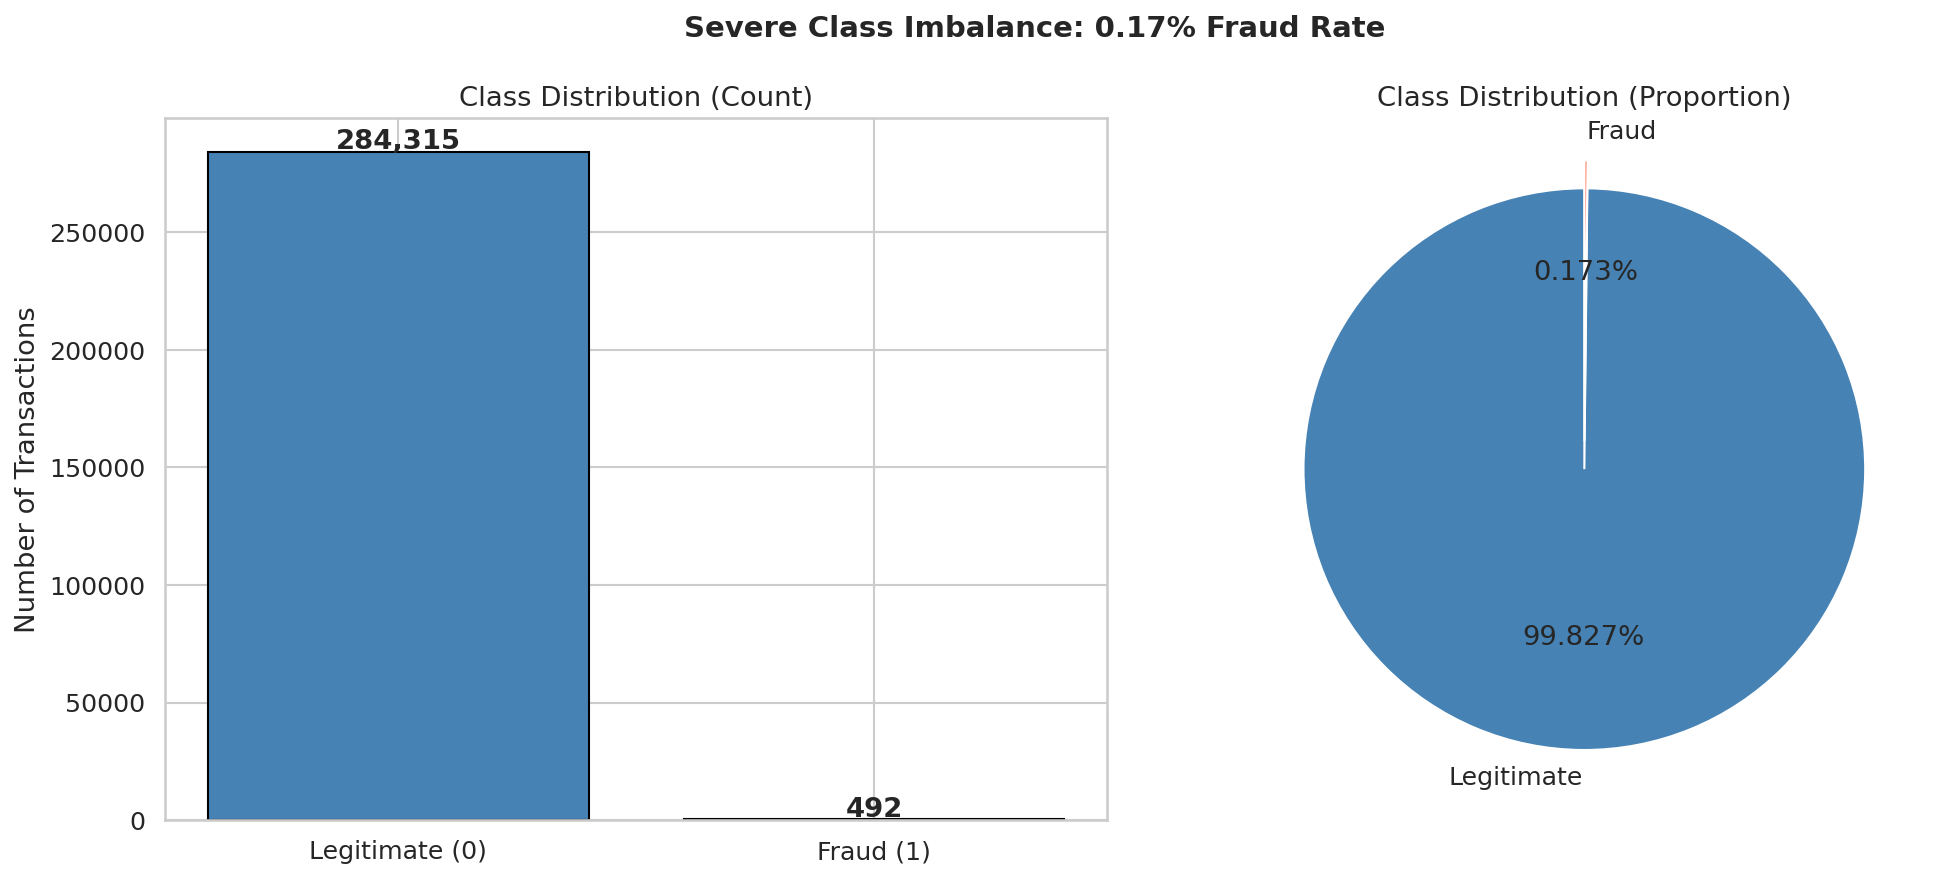
\includegraphics[width=\columnwidth]{class_distribution.png}
\caption{Class distribution showing the severe imbalance: 99.83\% legitimate vs. 0.17\% fraudulent transactions.}
\label{fig:class_dist}
\end{figure}

% ─────────────────────────────────────────────
%  4. METHODOLOGY
% ─────────────────────────────────────────────
\section{Proposed Methodology}
\label{sec:methods}

We apply three classification algorithms that represent a spectrum from simple linear models to powerful ensemble methods, enabling a meaningful comparative analysis.

\subsection{Logistic Regression}

Logistic Regression (LR) models the probability of the positive class using the logistic function:

\begin{equation}
P(y=1 \mid \mathbf{x}) = \frac{1}{1 + e^{-(\mathbf{w}^T\mathbf{x} + b)}}
\end{equation}

where $\mathbf{w}$ is the weight vector and $b$ is the bias term, learned by maximizing the log-likelihood with L2 regularization. LR serves as an interpretable linear baseline.

\textbf{Configuration:} Regularization strength $C = 0.01$ (strong regularization to reduce overfitting), solver \texttt{lbfgs}, \texttt{class\_weight=`balanced'}, \texttt{max\_iter=1000}.

\textbf{Rationale:} LR is chosen as a baseline because its linear decision boundary makes it computationally efficient and its outputs are directly interpretable as probabilities. The \texttt{class\_weight=`balanced'} setting further compensates for class imbalance at the algorithm level.

\subsection{Random Forest}

Random Forest (RF) \cite{breiman2001} is an ensemble method that builds multiple decision trees on bootstrapped subsets of the training data and aggregates their predictions by majority vote:

\begin{equation}
\hat{y} = \text{mode}\{h_t(\mathbf{x})\}_{t=1}^{T}
\end{equation}

where $h_t$ is the $t$-th decision tree trained on a random subset of features at each split, and $T$ is the number of trees.

\textbf{Configuration:} $T = 200$ trees, \texttt{max\_depth=20}, \texttt{min\_samples\_split=5}, \texttt{min\_samples\_leaf=2}, \texttt{class\_weight=`balanced'}.

\textbf{Rationale:} RF was selected for its robustness to outliers, ability to model non-linear feature interactions, and native feature importance estimation. The balanced class weight further mitigates imbalance at the tree level.

\subsection{XGBoost}

XGBoost \cite{chen2016} is a gradient boosting framework that builds an additive ensemble of weak learners (shallow trees) by iteratively minimizing a regularized loss function:

\begin{equation}
\mathcal{L}^{(t)} = \sum_{i=1}^{n} l(y_i, \hat{y}_i^{(t-1)} + f_t(\mathbf{x}_i)) + \Omega(f_t)
\end{equation}

where $f_t$ is the $t$-th tree, $l$ is the log-loss, and $\Omega$ is a regularization term penalizing tree complexity.

\textbf{Configuration:} \texttt{n\_estimators=300}, \texttt{max\_depth=6}, \texttt{learning\_rate=0.05}, \texttt{subsample=0.8}, \texttt{colsample\_bytree=0.8}, \texttt{scale\_pos\_weight=1.0} (SMOTE already balances training data).

\textbf{Rationale:} XGBoost is included as a state-of-the-art gradient boosting method known for strong performance on tabular data, second-order optimization, and built-in regularization to prevent overfitting.

% ─────────────────────────────────────────────
%  5. EXPERIMENTAL RESULTS
% ─────────────────────────────────────────────
\section{Experimental Results and Discussion}
\label{sec:results}

\subsection{Experimental Setup}

All experiments were conducted in Python 3.13 using scikit-learn 1.3+, XGBoost 2.0+, and imbalanced-learn 0.11+. Models were trained on the SMOTE-balanced training set (453,204 samples) and evaluated on the original-distribution test set (56,746 samples, 95 fraud cases) to simulate real-world deployment. A fixed random seed of 42 was used throughout for reproducibility.

\subsection{Evaluation Metrics}

Given the severe class imbalance, we justify our choice of five complementary metrics:

\begin{itemize}
    \item \textbf{Accuracy} — overall correctness; misleading alone due to imbalance.
    \item \textbf{Precision} — fraction of flagged transactions that are truly fraudulent; minimizes customer disruption from false alarms.
    \item \textbf{Recall (Sensitivity)} — fraction of actual fraud cases detected; minimizes financial losses from missed fraud.
    \item \textbf{F1-Score} — harmonic mean of Precision and Recall; primary metric for imbalanced classification.
    \item \textbf{ROC-AUC} — area under the ROC curve; measures discrimination ability across all decision thresholds.
\end{itemize}

\subsection{Results}

Table~\ref{tab:results} presents the complete evaluation results for all three models.

\begin{table}[H]
\centering
\caption{Comparative Performance Results}
\label{tab:results}
\begin{tabular}{lccccc}
\toprule
\textbf{Model} & \textbf{Acc.} & \textbf{Prec.} & \textbf{Rec.} & \textbf{F1} & \textbf{AUC} \\
\midrule
Logistic Regression & 0.9741 & 0.0539 & \textbf{0.8737} & 0.1015 & 0.9618 \\
Random Forest       & \textbf{0.9994} & \textbf{0.8391} & 0.7684 & \textbf{0.8022} & \textbf{0.9842} \\
XGBoost             & 0.9987 & 0.5778 & 0.8211 & 0.6783 & 0.9733 \\
\bottomrule
\end{tabular}
\end{table}

\begin{figure}[H]
\centering
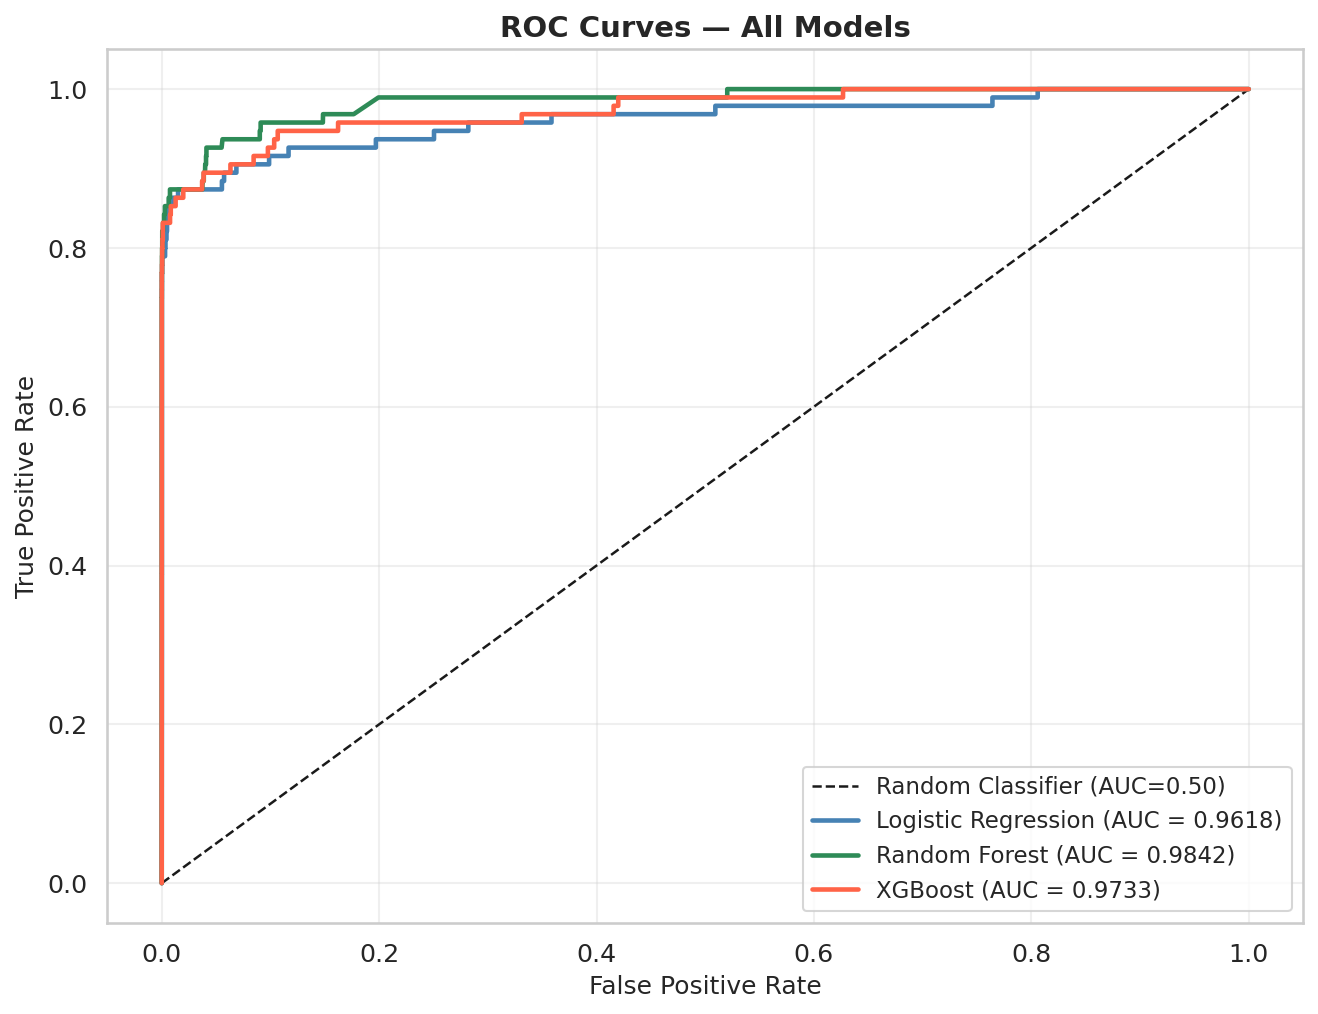
\includegraphics[width=\columnwidth]{roc_curves_combined.png}
\caption{ROC curves for all three models. Random Forest achieves the highest AUC (0.9842), indicating superior discrimination between fraud and legitimate transactions across all thresholds.}
\label{fig:roc}
\end{figure}

\begin{figure}[H]
\centering
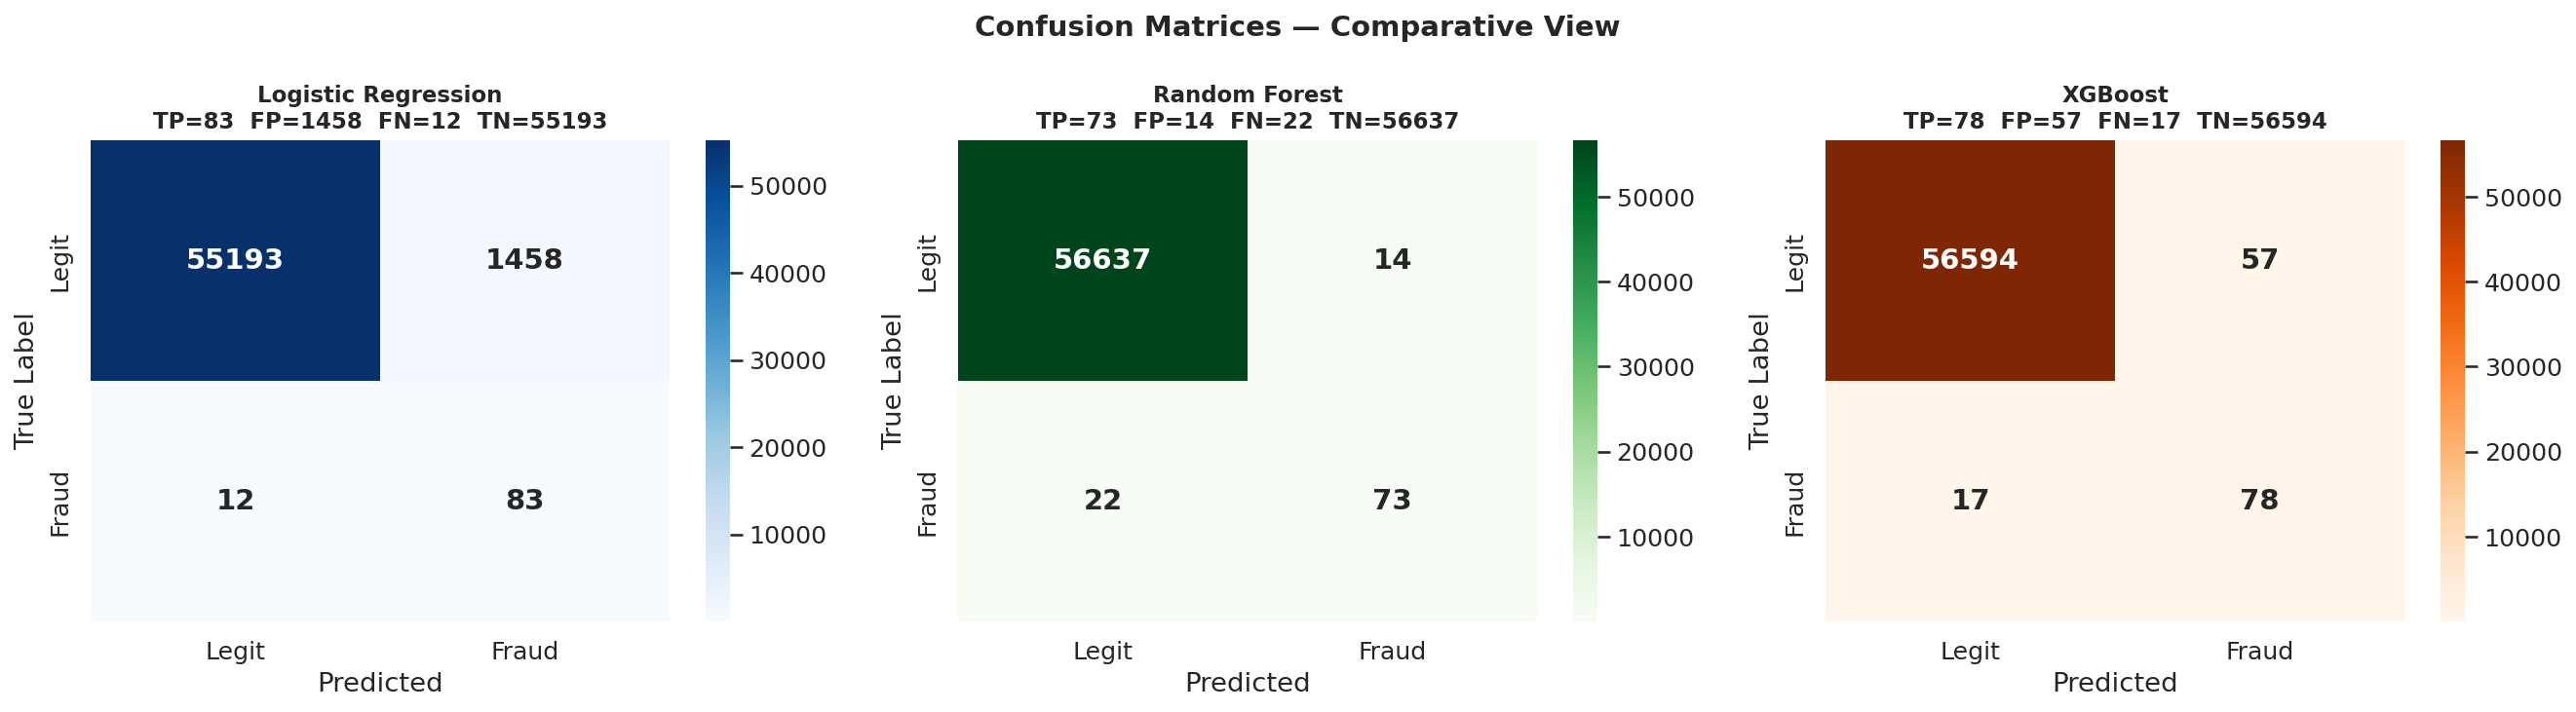
\includegraphics[width=\columnwidth]{confusion_matrices_combined.png}
\caption{Confusion matrices for all three models. LR flags many legitimate transactions as fraud (low precision). RF achieves the best balance with 73 true positives and only 14 false positives. XGBoost detects 78 fraud cases with 57 false positives.}
\label{fig:cm}
\end{figure}

\begin{figure}[H]
\centering
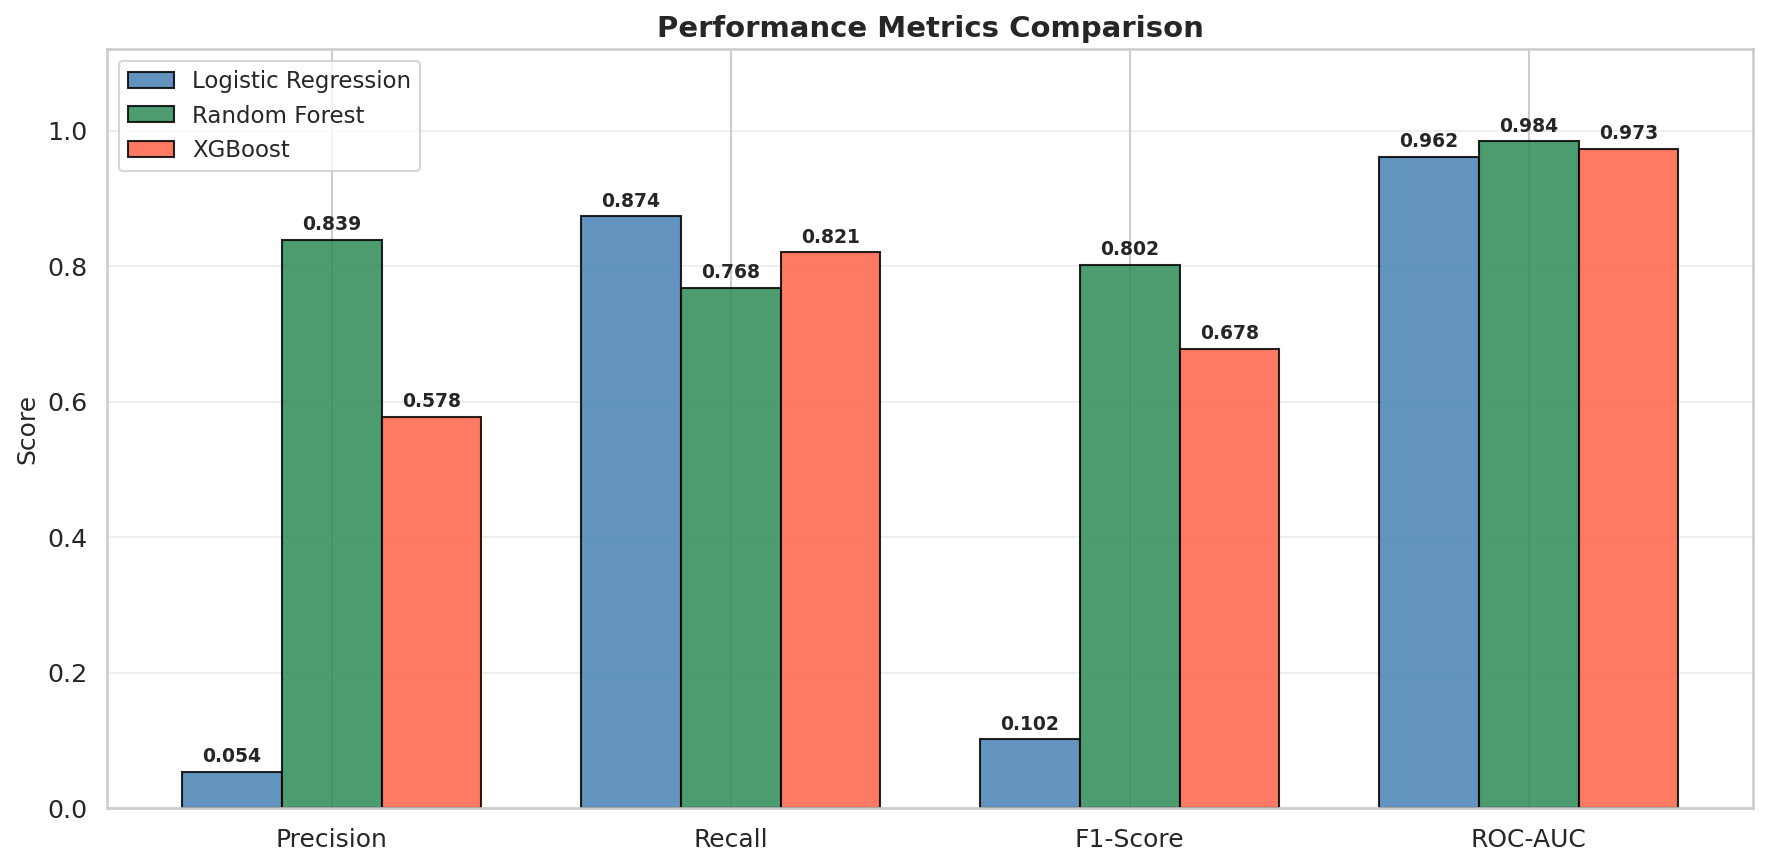
\includegraphics[width=\columnwidth]{metrics_comparison_bar.png}
\caption{Comparative bar chart of Precision, Recall, F1-Score, and ROC-AUC across all models. Random Forest dominates in Precision, F1, and AUC.}
\label{fig:metrics_bar}
\end{figure}

\subsection{Feature Importance Analysis}

\begin{figure}[H]
\centering
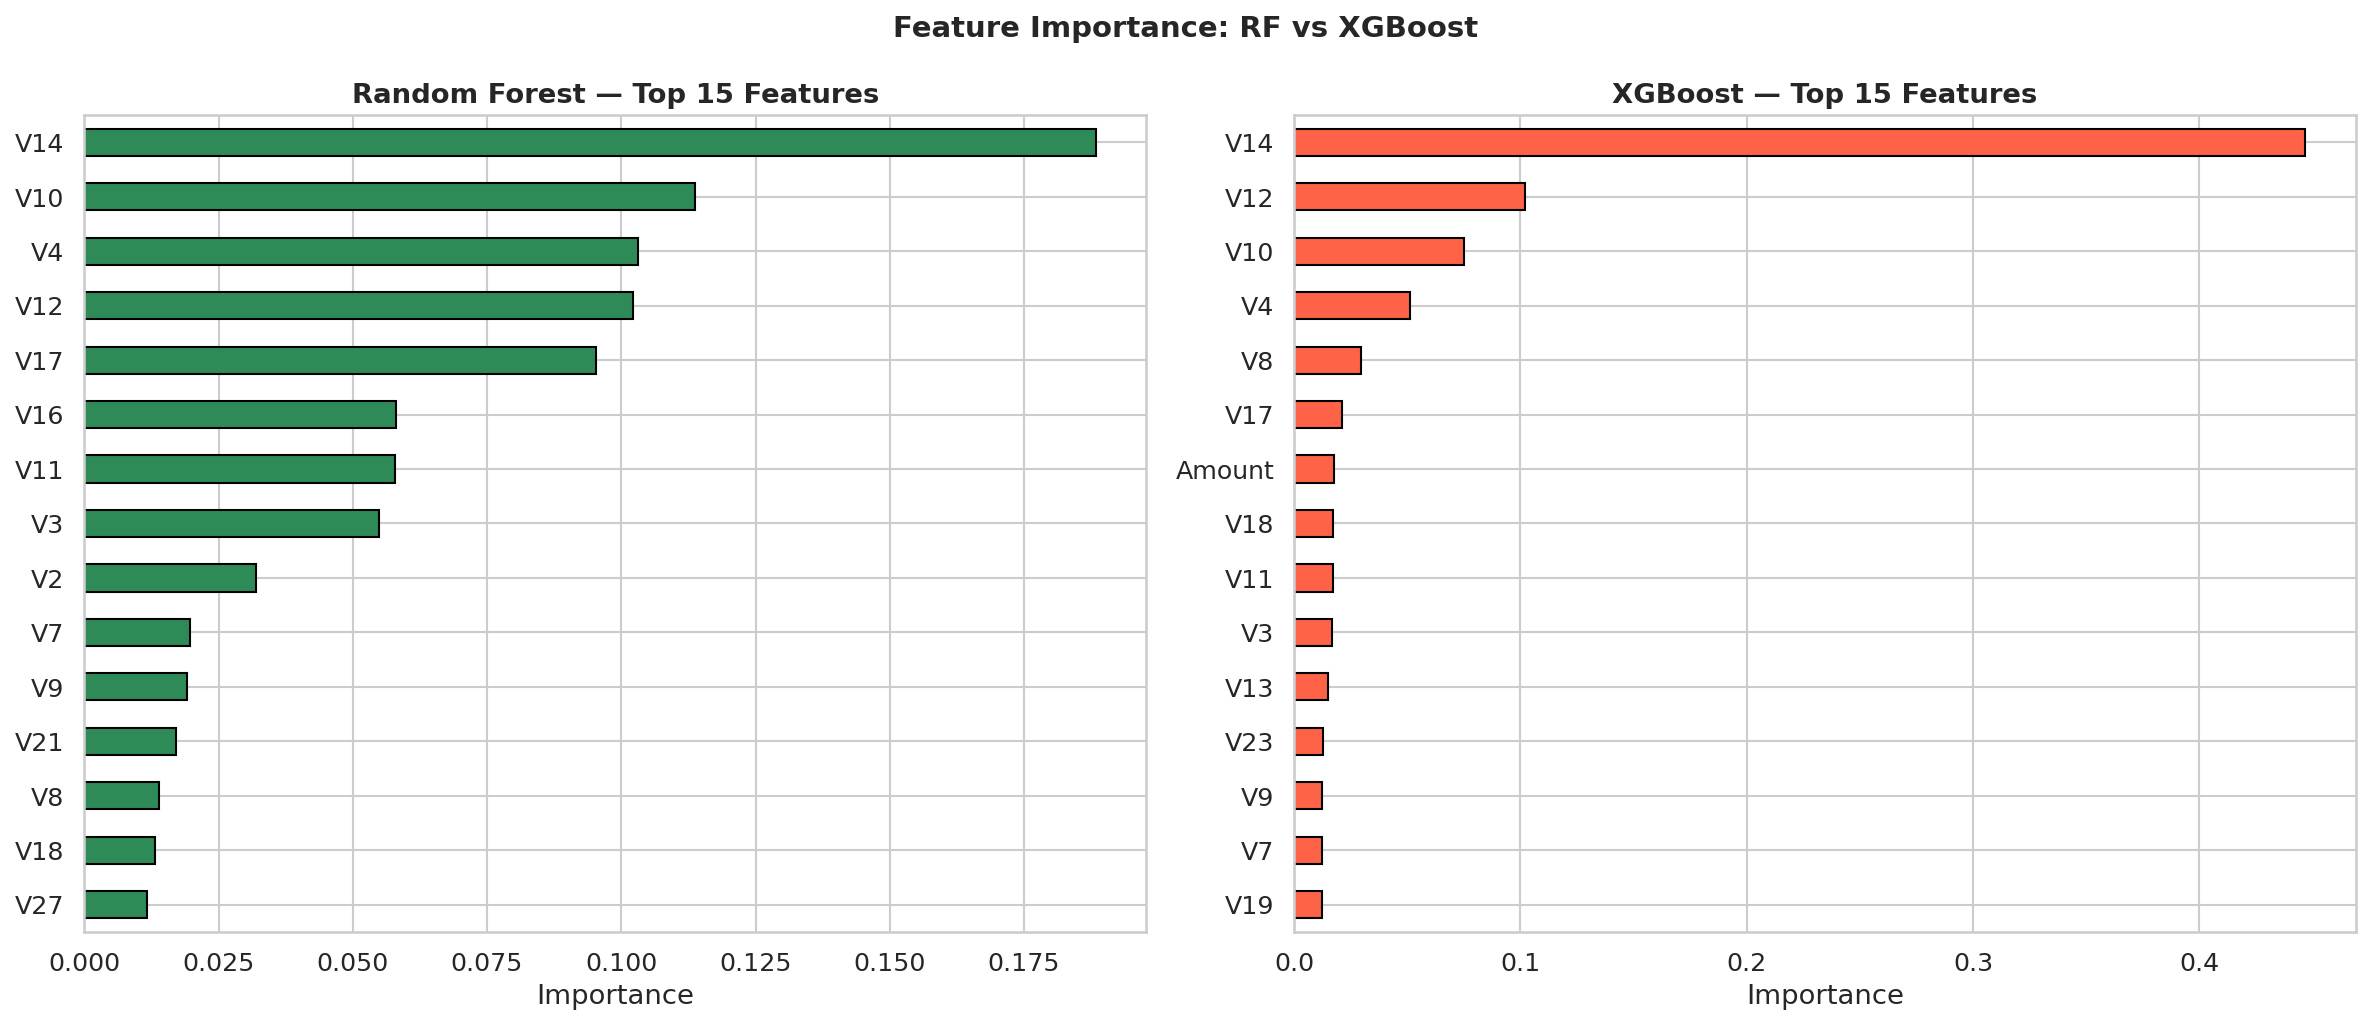
\includegraphics[width=\columnwidth]{feature_importance_comparison.png}
\caption{Feature importance from Random Forest and XGBoost. Both models consistently rank V14, V10, V12, and V4 among the most discriminative features, indicating robustness of these PCA components as fraud indicators.}
\label{fig:feat_imp}
\end{figure}

Both ensemble methods agree on the top discriminative features: V14 (most important in XGBoost with 44.7\% contribution), V10, V12, V4, and V17. This consistent ranking across independently trained models validates the reliability of these PCA components as fraud signals.

\subsection{Discussion}

\textbf{Random Forest} achieves the best overall performance with the highest F1-Score (0.8022) and ROC-AUC (0.9842). Its high precision (0.8391) is particularly valuable in production systems, where false alarms lead to customer dissatisfaction and operational costs. The ensemble mechanism effectively reduces variance and the balanced class weight at the tree level provides additional imbalance robustness.

\textbf{XGBoost} achieves the highest recall (0.8211) among the ensemble methods, detecting more fraud cases at the cost of more false positives (precision = 0.5778). This trade-off may be acceptable in high-stakes scenarios where missing a fraud case is more costly than a false alarm. Further hyperparameter tuning (particularly adjusting \texttt{scale\_pos\_weight} and decision threshold) could improve its precision without significantly reducing recall.

\textbf{Logistic Regression} achieves the highest recall (0.8737) overall but extremely low precision (0.0539), effectively flagging most transactions as suspicious. This behavior stems from the model's linear decision boundary in a non-linearly separable feature space. While unusable in isolation as a production classifier, its strong ROC-AUC (0.9618) confirms that linear separability exists in the feature space, and it serves as a valuable interpretable baseline that justifies the use of ensemble methods.

The severe class imbalance (1:578 ratio) is a defining challenge of this dataset. Our results demonstrate that SMOTE combined with class-weight balancing is effective: all three models achieve recall well above 0.75, meaning at least 75\% of actual fraud is detected. The choice between models ultimately depends on the business cost function: if false negatives (missed fraud) are more costly, XGBoost's higher recall may be preferred; if false positives (frozen cards, customer complaints) are more costly, Random Forest's superior precision is the right choice.

% ─────────────────────────────────────────────
%  6. CONCLUSION
% ─────────────────────────────────────────────
\section{Conclusion}
\label{sec:conclusion}

This paper presented a comparative study of three supervised classification methods for credit card fraud detection on a real-world, large-scale imbalanced dataset. We demonstrated that:

\begin{enumerate}
    \item Random Forest achieves the best overall performance (F1 = 0.8022, AUC = 0.9842) and is the recommended model for production deployment where precision is critical.
    \item XGBoost provides a strong alternative with higher recall (0.8211), suitable when minimizing missed fraud is the priority.
    \item Logistic Regression, while impractical as a standalone classifier due to near-zero precision, confirms linear separability in the feature space and serves as an important interpretable baseline.
    \item SMOTE oversampling applied exclusively to the training set effectively addresses class imbalance without introducing data leakage.
    \item Features V14, V10, V12, and V4 are consistently identified as the most discriminative across both ensemble methods.
\end{enumerate}

\textbf{Limitations and Future Work:} This study uses PCA-transformed features, limiting interpretability of feature importance. Future work could explore: (1) threshold optimization per business cost function, (2) time-aware train/test splits to simulate concept drift, (3) deep learning approaches (autoencoders, LSTM) for anomaly-based detection, and (4) online/streaming fraud detection to handle evolving fraud patterns in real time.

% ─────────────────────────────────────────────
%  TOOLS AND LIBRARIES
% ─────────────────────────────────────────────
\section*{Tools and Libraries}

All experiments were implemented in Python 3.13. Key libraries used: \texttt{scikit-learn} 1.3+ for Logistic Regression, Random Forest, preprocessing and metrics; \texttt{XGBoost} 2.0+ for gradient boosting; \texttt{imbalanced-learn} 0.11+ for SMOTE; \texttt{pandas} and \texttt{numpy} for data manipulation; \texttt{matplotlib} and \texttt{seaborn} for visualization. Source code and dataset link are available in the project repository.

% ─────────────────────────────────────────────
%  REFERENCES
% ─────────────────────────────────────────────
\begin{thebibliography}{00}

\bibitem{nilson2023}
The Nilson Report, ``Payment Card Fraud Losses Worldwide,'' HSN Consultants, Inc., 2023.

\bibitem{dal2015}
A. Dal Pozzolo, O. Caelen, R. A. Johnson, and G. Bontempi, ``Calibrating probability with undersampling for unbalanced classification,'' in \textit{Proc. IEEE Symp. Comput. Intell. Data Mining}, 2015, pp. 159--166.

\bibitem{bolton2002}
R. J. Bolton and D. J. Hand, ``Statistical fraud detection: A review,'' \textit{Statistical Science}, vol. 17, no. 3, pp. 235--255, 2002.

\bibitem{bhattacharyya2011}
S. Bhattacharyya, S. Jha, K. Tharakunnel, and J. C. Westland, ``Data mining for credit card fraud: A comparative study,'' \textit{Decision Support Systems}, vol. 50, no. 3, pp. 602--613, 2011.

\bibitem{breiman2001}
L. Breiman, ``Random forests,'' \textit{Machine Learning}, vol. 45, no. 1, pp. 5--32, 2001.

\bibitem{chen2016}
T. Chen and C. Guestrin, ``XGBoost: A scalable tree boosting system,'' in \textit{Proc. 22nd ACM SIGKDD Int. Conf. Knowl. Discovery Data Mining}, 2016, pp. 785--794.

\bibitem{makki2019}
S. Makki, Z. Assaghir, Y. Taher, R. Haque, M.-S. Hacid, and H. Zeineddine, ``An experimental study with imbalanced classification approaches for credit card fraud detection,'' \textit{IEEE Access}, vol. 7, pp. 93010--93022, 2019.

\bibitem{chawla2002}
N. V. Chawla, K. W. Bowyer, L. O. Hall, and W. P. Kegelmeyer, ``SMOTE: Synthetic minority over-sampling technique,'' \textit{J. Artif. Intell. Res.}, vol. 16, pp. 321--357, 2002.

\bibitem{fernandez2018}
A. Fernández, S. García, F. Herrera, and N. V. Chawla, ``SMOTE for learning from imbalanced data: Progress and challenges, marking the 15-year anniversary,'' \textit{J. Artif. Intell. Res.}, vol. 61, pp. 863--905, 2018.

\bibitem{dataset2018}
ULB Machine Learning Group, ``Credit Card Fraud Detection Dataset,'' Kaggle, 2018. [Online]. Available: \url{https://www.kaggle.com/datasets/mlg-ulb/creditcardfraud}

\end{thebibliography}

\end{document}
